\subsubsection{Digit tops}
The {\dtop} gadgets have specific geometry, such that they allow {\firstwarp} and
{\secondwarp} units to ``wake up" and end their warp journey. A {\dtop} is placed on
the north end of a digit. These hold a increment/copy signal and the regional index
of the next digit to read.
\vspace{1cm}

For each {\inc} $\in \{ {\tt increment, copy } \}$
\begin{itemize}
    \item General digit tops common to all assemblies

    \begin{figure}[H]
        \centering
        \begin{subfigure}[t]{0.2\textwidth}
            \centering
            \includegraphics[width=0.2\textwidth]{digit_tops/digit_top_general}
            \caption{\label{fig:digit_tops/digit_top_general} General }
        \end{subfigure}%
        ~
    \end{figure}

    \begin{itemize}
        \item Create
        $\begin{aligned}[t]
            \dtop(& \left \langle {\tt DigitTopDigit1}, \inc \right\rangle, & \\
                    & \left \langle {\tt ReturnD1ReadD2}, \inc \right\rangle \;)
        \end{aligned}$
        \vspace{.5cm}

        \item Create
        $\begin{aligned}[t]
            \dtop(& \left \langle {\tt DigitTopDigit2}, \inc \right\rangle, & \\
                    & \left \langle {\tt ReturnD2ReadD3}, \inc \right\rangle \;)
        \end{aligned}$
        \vspace{.5cm}

        \item Create
        $\begin{aligned}[t]
            \dtop(& \left \langle {\tt DigitTopDigit3}, \inc \right\rangle,  \\
                    & \left \langle {\tt ReturnD3ReadD1}, \inc \right\rangle \;)
        \end{aligned}$

    \end{itemize}


    \item MSR-specific digit tops. The first tile placed in all digit top gadgets is the rightmost, bottommost tile.

    \begin{figure}[H]
        \centering
        \begin{subfigure}[t]{0.2\textwidth}
            \centering
            \includegraphics[width=0.2\textwidth]{digit_tops/digit_top_case1_digit1_msr}
            \caption{\label{fig:digit_tops/digit_top_case1_digit1_msr} Digit 1 -- Case 1}
        \end{subfigure}%
        ~
        \begin{subfigure}[t]{0.2\textwidth}
            \centering
            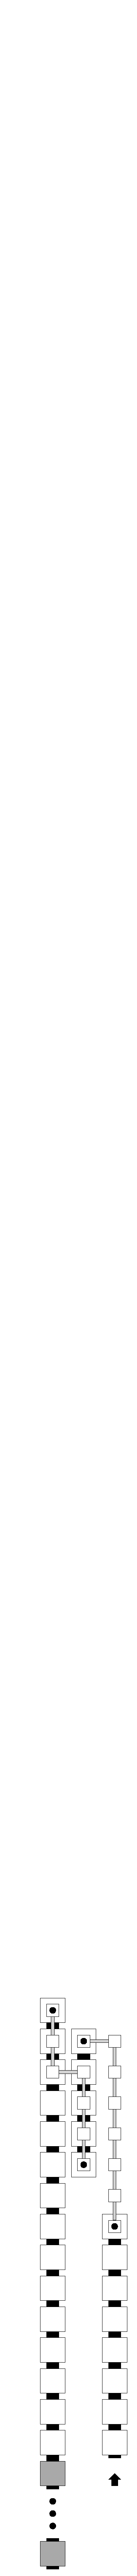
\includegraphics[width=0.2\textwidth]{digit_tops/digit_top_case2_digit1_msr}
            \caption{\label{fig:digit_tops/digit_top_case2_digit1_msr} Digit 1 -- Case 2}
        \end{subfigure}%
        ~
        \begin{subfigure}[t]{0.2\textwidth}
            \centering
            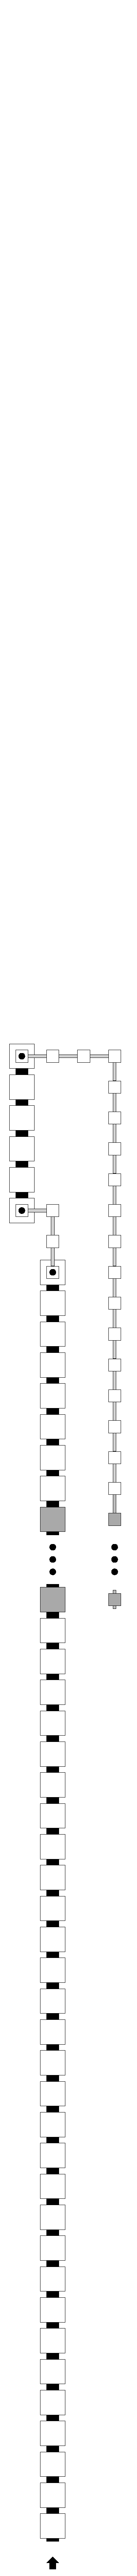
\includegraphics[width=0.2\textwidth]{digit_tops/digit_top_case2_digit2_msr}
            \caption{\label{fig:digit_tops/digit_top_case2_digit2_msr} Digit 2 -- Case 2}
        \end{subfigure}%
        ~
        \begin{subfigure}[t]{0.2\textwidth}
            \centering
            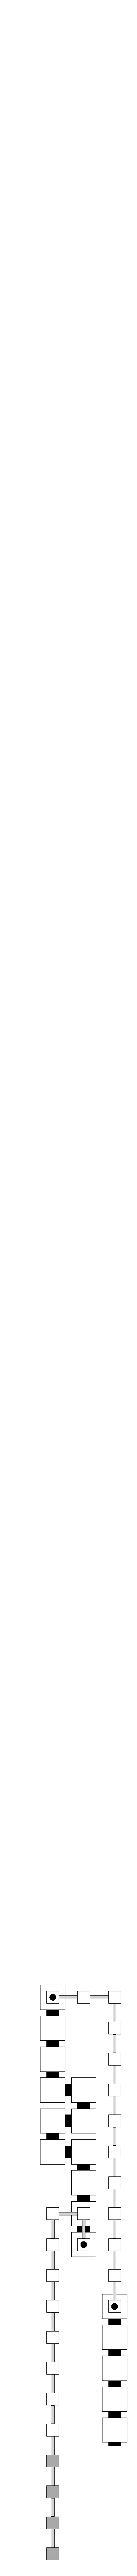
\includegraphics[width=0.2\textwidth]{digit_tops/digit_top_case3_msr}
            \caption{\label{fig:digit_tops/digit_top_case3_msr} All digits -- Case 3}
        \end{subfigure}%
    \end{figure}


    \begin{enumerate}[label=\alph*)]
        % For digit 1, case 1
        \item if $i$ is 1 and MSR contains 1 digit and $l$ starts with 11:

        Create
        $\begin{aligned}[t]
            \dtopdonecaseone(& \left \langle {\tt DigitTopDigit1-Case1}, \inc \right\rangle, & \\
                                & \left \langle {\tt ReturnD1ReadNextRow},  \inc \right\rangle \;)
        \end{aligned}$
        \vspace{.5cm}


        % For digit 1, case 2
        \item if $i$ is 1 and MSR contains 2 digits and $l$ starts with 01:

        Create
        $\begin{aligned}[t]
            \dtopdonecasetwo(& \left \langle {\tt DigitTopDigit1-Case2}, \inc \right\rangle, & \\
                                & \left \langle {\tt ReturnD1ReadD2-Case2}, \inc \right\rangle \;)
        \end{aligned}$
        \vspace{.5cm}


        % For digit 2, case 2
        \item if $i$ is 2 and MSR contains 2 digits and $l$ starts with 11:

        Create
        $\begin{aligned}[t]
            \dtopdtwocasetwo(& \left \langle {\tt DigitTopDigit2-Case2}, \inc \right\rangle, & \\
                                & \left \langle {\tt ReturnD2ReadNextRow},  \inc \right\rangle \;)
        \end{aligned}$
        \vspace{.5cm}


        % For digit 3, in case 3
        \item if $i$ is 3 and MSR contains 3 digits and $l$ starts with 11:

        Create
        $\begin{aligned}[t]
            \dtopcasethree(& \left \langle {\tt DigitTop-Case3},      \inc \right\rangle, & \\
                            & \left \langle {\tt ReturnD3ReadNextRow}, \inc \right\rangle \;)
        \end{aligned}$
        \vspace{.5cm}


    \end{enumerate}

\end{itemize}
\vspace{1cm}